	% !TEX spellcheck = en_US

\section{Supplementary Materials}


	\subsection{Response Symmetry in GLMs}
		\normalsize
		In the univariate significance tests of  GLM$_{mv}$s, species with optima at the middle of an uni- or bimodal gradient were assigned high \textit{p}-values. 
		%
		Here, I will show that this likely occurred due to the symmetry of the response shape when considered over the whole sampling range. 
		%
		Figure \ref{fig:uniglm} shows three unimodal responses that only differ in the position of their optimum. One (orange) is at 50 which is exactly the middle of the sampled gradient, as is indicated by the dashed line, one (blue) is at 49 and the last (green) at 25. 
		
		% ---------------------------------------------------------------------------- %
		%& Figure: Unimodal response shapes and corresponding regression coefficients
		% ---------------------------------------------------------------------------- %
		
		\begin{figure}[h!]
			\centering
			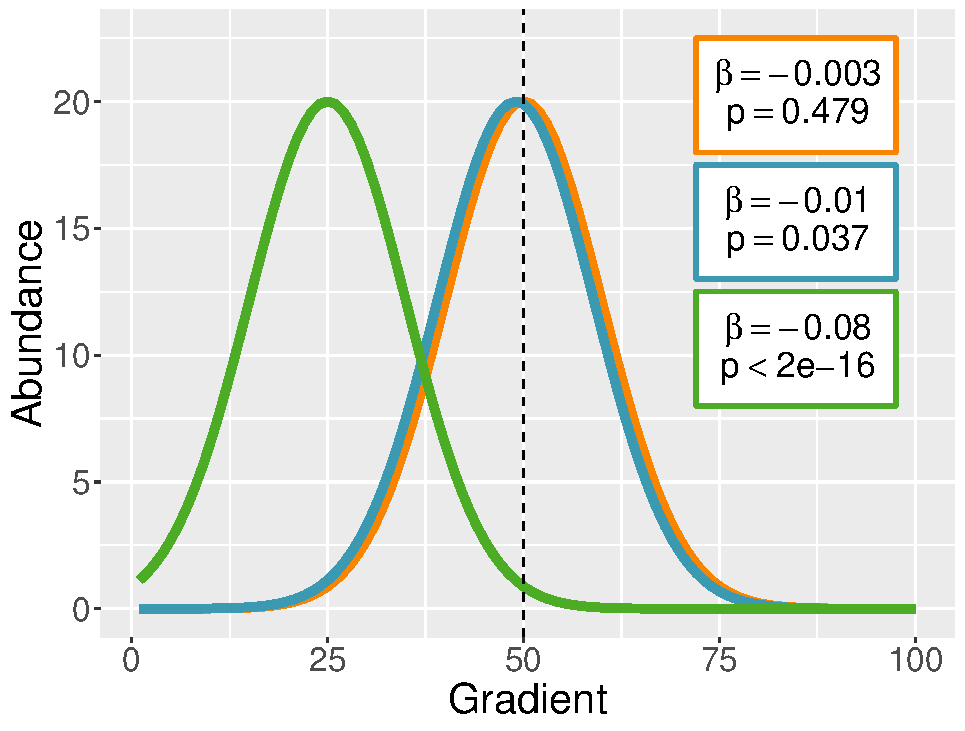
\includegraphics[width=0.5\linewidth]{../02_Figures/uniglm}
			\caption{
					Unimodal response shapes with different optima.
					%
					The dashed line indicates the middle of the sampled range.
					%	
					Each color represents a different species.
					%
					The response shapes only differ in the location of their optimum, both tolerance and maximal abundance are equal.
					%
					$\beta$ refers to the regression coefficient for the gradient in a GLM which models abundance as a function of the gradient and p to the corresponding \textit{p}-value.
					%
					The color of the boxes indicates which curve the values belong to.
					%
					The regression coefficient increase and the \textit{p}-values decrease as the distance of the optimum from the middle of the gradient increases.  
					}
			\label{fig:uniglm}
		\end{figure}
		   
		The \textit{p}-values and regression coefficients come from a GLM with negative binomial residual distribution, conducted with the MASS R-package \citep{Venables2002}.
		%
		The small difference in optima between the orange and the blue species entails a big disparity in regression coefficients. 
		%
		The regression coefficient of the blue species is approximately three times higher and the \textit{p}-value is less than a tenth of the orange ones.
		%
		The green species shows that the regression coefficient further increases and the \textit{p}-value further decreases as the optimum is farther removed from the middle. 
		%
		These results were comparable but not identical to those obtained when using optima higher than 50 (not shown here).\\
		
		% ---------------------------------------------------------------------------- %
		%& Figure: Bimodal response shapes and corresponding regression coefficients
		% ---------------------------------------------------------------------------- %
		
		\begin{figure}[h!]
			
			\begin{subfigure}{0.5\textwidth}
				\centering
				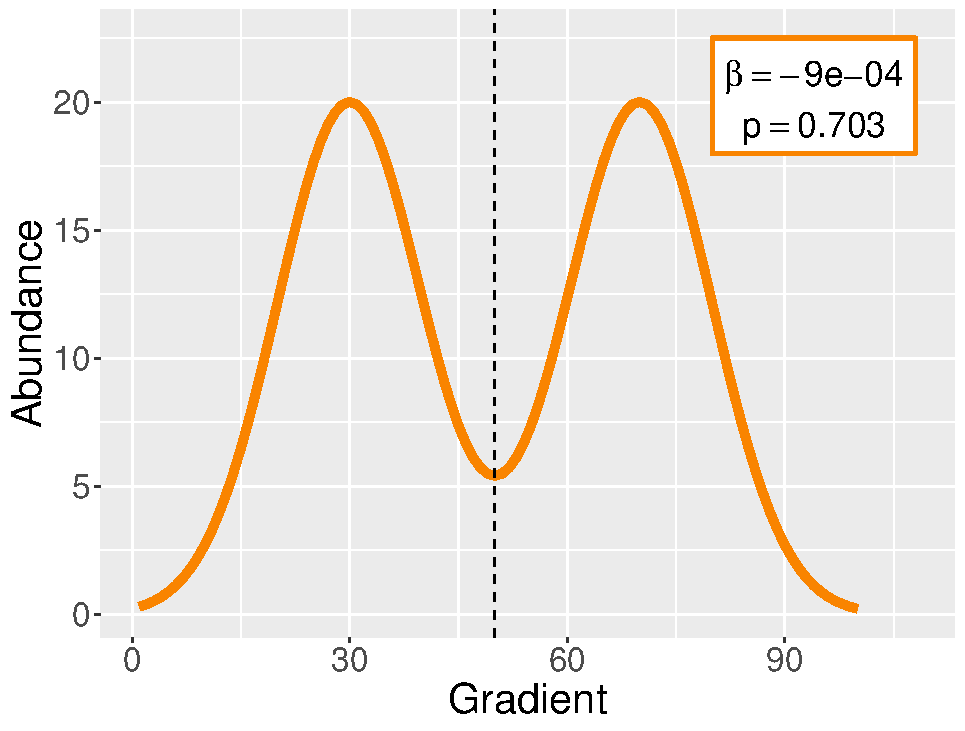
\includegraphics[width=1\linewidth]{../02_Figures/bi1}
				\caption{}
				\label{fig:biglm1}
			\end{subfigure}
			\begin{subfigure}{0.5\textwidth}
				\centering
				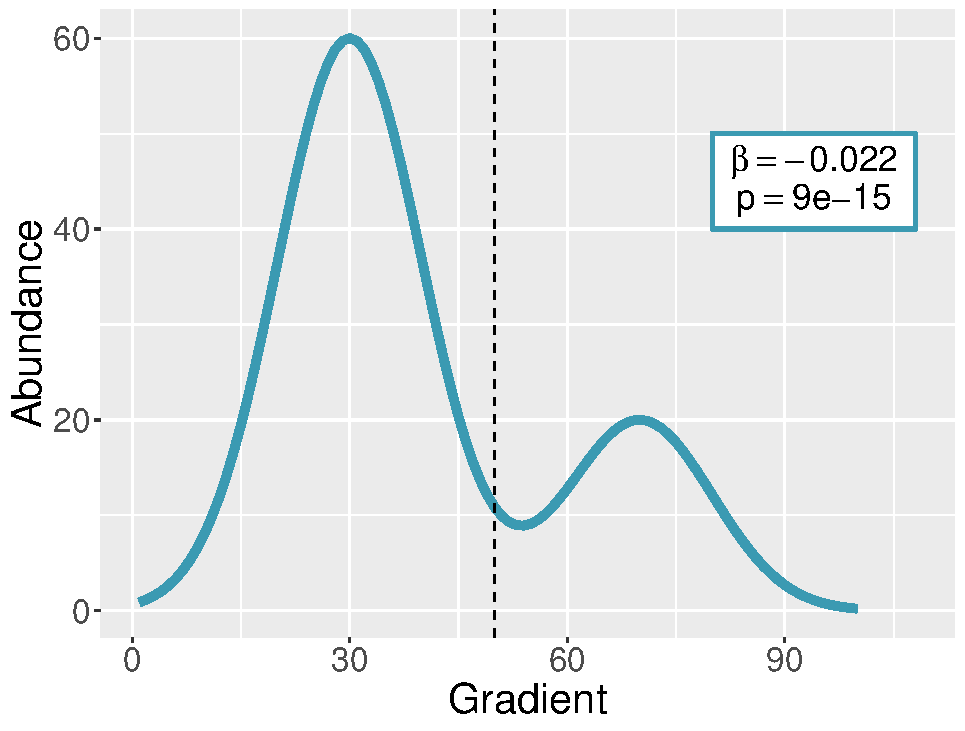
\includegraphics[width=1\linewidth]{../02_Figures/bi2}
				\caption{}
				\label{fig:biglm2}
			\end{subfigure}
			\begin{subfigure}{0.5\textwidth}
				\centering
				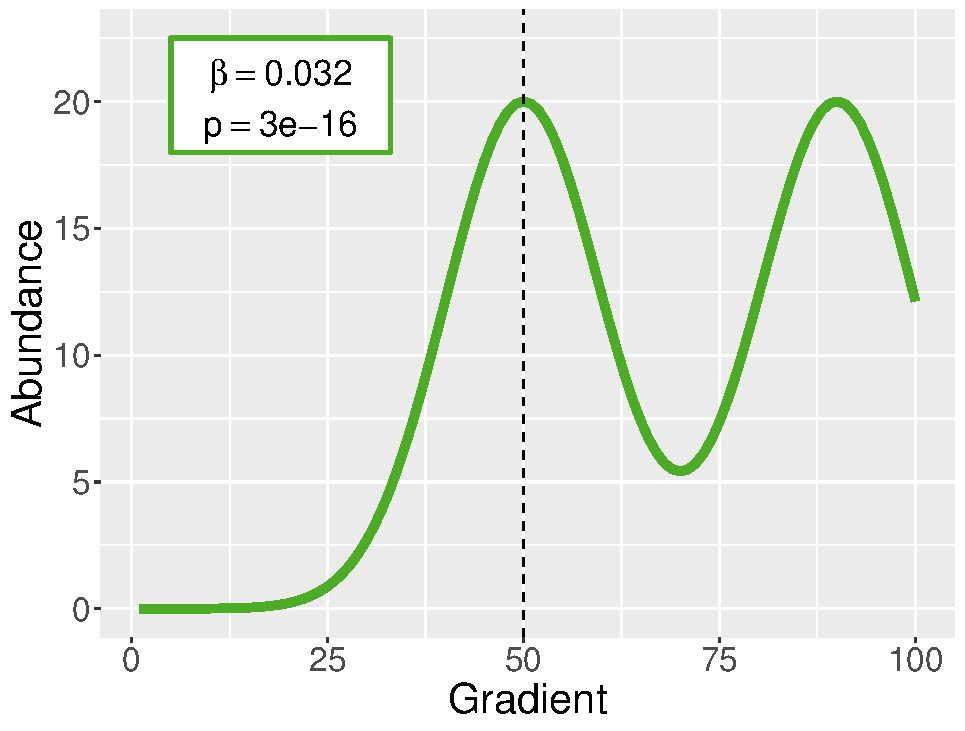
\includegraphics[width=1\linewidth]{../02_Figures/bi3}
				\caption{}
				\label{fig:biglm3}
			\end{subfigure}
			\caption{
				Bimodal response shapes. 
				%
				In the boxes $\beta$ is the regression coefficient for the gradient in a GLM which models Abundance as a function of the gradient. 
				%
				p is the associated \textit{p}-value. 
				%
				The dashed line indicates the middle of the sampled range.
				%
				(\textbf{a}) shows a symmetrical response, $\beta$ is low and the \textit{p}-value is high. 
				%
				(\textbf{b}) and (\textbf{c}) are asymmetrical modifications of (\textbf{a}). 
				%
				In (\textbf{b}) the maximum of the first optimum is higher than the second. 
				%
				This results in a higher $\beta$ and lower \textit{p}-value. 
				%
				(\textbf{c}) shows the same response shape as (\textbf{a}) but shifted to the right. 
				%
				This modification also results in a higher $\beta$ and lower \textit{p}-value.
			}
			\label{fig:biglm}
		\end{figure}
		
		
		Figure \ref{fig:biglm} shows a similar setup for bimodal response shapes. In figure \ref{fig:biglm1} the response is symmetrical. 
		%
		The middle of the gradient lies exactly between the two optima.
		%
		A GLM with negative binomial residual distribution returns a low regression coefficient (- 9e-04) and an appropriately high \textit{p}-value (0.703).
		%
		For figure \ref{fig:biglm2}, the maximal abundance at the first optimum was increased to three times that of the second.
		%
		The middle of the response shape still coincides with that of the gradient.
		%
		The regression coefficient (-0.22) is increased (in absolute terms) relative to the first model and the \textit{p}-value (9e-15) is decreased. 
		%
		A similar pattern can be observed when the response shape of figure \ref{fig:biglm1} is shifted to the right, as is done in figure \ref{fig:biglm3}.
		%
		Again, the regression coefficient (0.032) is increased and the \textit{p}-value (3e-16) decreased.\\
		
		These examples show that the symmetry of the response shape over the whole sampling range leads to small regression coefficients and the corresponding high \textit{p}-values. 
		%
		They also demonstrated that already small deviations from this symmetry (1/100 of the gradient length as the blue species in Figure \ref{fig:uniglm}) substantially increases the coefficient and decreases the \textit{p}-value.  
	
		
	
	\subsection{Further Details on Simulations} 
	
		The Table \ref{tab:SimDet} shows the model parameters used in the simulation.
		
		% ------------------------- %
		%& Table: Model parameters 
		% ------------------------- %
		\begin{table*}[h]
			\small
			\centering
			\caption{Model parameters used in simulations. An x indicates that the parameter is not relevant to the gradient types used. \textit{c} is the maximal abundance, \textit{t} the tolerance, \textit{u} the location of the optimum, $x_0$ the midway points of the sigmoid, $\beta$ the  linear response parameter and \textit{k} the steepness of the logistic curve. Values in braces are optima pairs for bimodal gradients.}
			\begin{tabular}{@{}llllll@{}}
				\toprule
				        & \textit{c} & \textit{t} & \textit{u}/ $x_0$                                 & $\beta$                & \textit{k}     \\
				\hline       
				Uni-Uni & 100 & 7.5 & 20, 50, 80                                                & x                   		  & x     \\
				Uni-Li  & 100 & 7.5 & 0, 25, 50, 75, 100                                        & 1, 1.2, 1.4, 1.6, 1.8       & x     \\
				Uni-Lo  & 100 & 7.5 & 20, 50, 80                                                & x                   		  & 0.1 \\
				Uni-Bi  & 100 & 5   & 20, 50, 80/ \{10, 30\}, \{40, 60\}, \{70, 90\}                        & x                  		  & x  \\
				Li-Li   & x   & x   & x                                                         & 80, 100, 120, 0.8, 1.1, 1.2 & x     \\
				Li-Lo   & 100 & x   & 15, 30, 45, 60, 75                                        & 0.1                   	  & 0.05  \\
				Li-Bi   & 100 & 6   & \{5, 25\}, \{25, 45\}, \{35, 55\}, \{55, 75\}, \{75, 95\} & 0.1                    	  & x     \\
				Lo-Lo   & 100 & x   & 20, 50, 80                                                & x                     	  & 0.1   \\
				Lo-Bi   & 100 & 6   & 20, 50, 80/ \{5, 25\}, \{35, 55\}, \{75, 95\}             & x                      	  & 0.1   \\
				Bi-Bi   & 100 & 6   & \{5, 25\}, \{35, 55\}, \{75, 95\}                         & x                      	  & x     \\
				\toprule
			\end{tabular}
			\label{tab:SimDet}
		\end{table*}
		\normalsize	
		The optimum parameter \textit{u} is the only instance of a parameter that is relevant to both gradients and differing between them. 
		%
		The different values are separated by forward slashes. 
		%
		Bimodal gradients require two optima per species. 
		%
		The used combinations are shown in braces. \\
		%
		In \textit{Li-Li}, the first three species reacted to \textit{env1} the next three to \textit{env2} and the last three to both.
		%
		For this reason, the $\beta$ parameters of the last three species are much lower than the first three. 
		%
		This also causes the high \textit{p}-values for \textit{env1} and \textit{env2} in \textit{Li-Li} (see Table \ref{tab:GLMUNI1}). 
		
	\subsection{Ordination Diagrams}
	
		As the result of dimension reduction, db-RDA, CCA, and CAO/CQO produce ordination diagrams. 
		%
		In the following section, a selection of diagrams will be presented for all four methods. \\ 
		%
		This selection will include the models: \textit{Uni-Uni}, \textit{Uni-Li}, \textit{Li-Li} and \textit{Lo-Lo}.
		%
		The first diagrams are from the db-RDA analyses (Figure \ref{fig:smdbord}). 
		%
		All subplots include explanatory variables (blue arrows), species scores (red letters), site scores as linear combinations of explanatory variables (grey points, LC-scores) and sites scores as weighted averages of species scores (green triangles, WA-scores).
		%
		These data are plotted in scaling 1 (distance-triplot) and can be interpreted as follows: 
		%
		i.) the angles between explanatory variables and the arrow that could be drawn from the centroid to each species score represent their correlation, %
		ii.) distances between objects approximate their Euclidean distance.\\
		%
		The species scores are positioned correctly in Figure \ref{fig:smdbord} a-c but in d the original pattern is not recognizable anymore. 
		%
		LC-scores always form  squares and the distance between the points is approximately constant. 
		%
		WA-scores are more prone to deformation. 
		%
		In \ref{fig:smdbord} a WA-scores are concentrated around species scores, in b they are fan-shaped, in c they look good and in d they appear to form a circle instead of a square.
		%
		In all models explanatory variables either load equally strong on both axes or each load on a separate axis.
	
		% ----------------------------------- %
		%& Figure: db-RDA ordination diagrams 
		% ----------------------------------- %
		\begin{figure}[h!]
			
			\begin{subfigure}{0.5\textwidth}		
					\centering
					\includegraphics[width=.55\linewidth]{"../02_Figures/dbRDASM1"}
					\caption{Uni-Uni}
			\end{subfigure}
			%
			\begin{subfigure}{0.5\textwidth}
					\centering		
					\includegraphics[width=.55\linewidth]{"../02_Figures/dbRDASM2"}
					\caption{Uni-Li}
			\end{subfigure}
			%
			\begin{subfigure}{0.5\textwidth}	
					\centering	
					\includegraphics[width=.55\linewidth]{"../02_Figures/dbRDASM3"}
					\caption{Li-Li}
			\end{subfigure}
			\begin{subfigure}{0.5\textwidth}		
					\centering
					\includegraphics[width=.55\linewidth]{"../02_Figures/dbRDASM4"}
					\caption{Lo-Lo}
			\end{subfigure}
			
			\caption{Triplots of the db-RDA analyses of (\textbf{a}) Uni-Uni, (\textbf{b)} Uni-Li, (\textbf{c}) Li-Li and (\textbf{d}) Lo-Lo. For every response combination the class 1 model was used.}
			\label{fig:smdbord}
			
		\end{figure}
	
		%& CCA
		
		Figure \ref{fig:smccaord} shows the triplots of the CCA analyses.
		%
		The same symbology as in Figure \ref{fig:smdbord} was used.
		%
		Again, scaling 1 is utilized.
		%
		In CCA this can be interpreted following these rules: 
		%
		i.) An orthogonal projection from an object (site or species score) on an explanatory variable approximates that object's position along that variable, ii.)  distances among object approximate their chi-squared distance. \\
		%
		In Figure \ref{fig:smccaord} a,c and d the species scores are placed correctly relative to the explanatory variables. 
		%
		In \textit{Uni-Li} they are only ordered along the unimodal gradient and the second axis is determined by noise variables.
		%
		The LC-scores form are square and are equidistant in \textit{Uni-Uni} and \textit{Lo-Lo}. 
		%
		In \textit{Uni-Li} they appear to be randomly distributed and in \textit{Li-Li} they are fan-shaped with the distance between points increasing towards lower values of the explanatory variables. 
		% 
		WA-scores are concentrated around species scores in \textit{Uni-Uni}, fan-shaped in \textit{Li-Li} and \textit{Lo-Lo} and scattered, though mostly absent in \textit{Uni-Li}. 
		In contrast to the db-RDA triplots, the species scores never lie outside the site scores. 
		
		% ----------------------------------- %
		%& Figure: CCA ordination diagrams 	
		% ----------------------------------- %		
		\begin{figure}[h]
			\begin{subfigure}{0.5\textwidth}		
				\centering
				\includegraphics[width=.8\linewidth]{"../02_Figures/CCASM1"}
				\caption{Uni-Uni}
			\end{subfigure}
			%
			\begin{subfigure}{0.5\textwidth}
				\centering		
				\includegraphics[width=.8\linewidth]{"../02_Figures/CCASM2"}
				\caption{Uni-Li}
			\end{subfigure}
			%
			\begin{subfigure}{0.5\textwidth}	
				\centering	
				\includegraphics[width=.8\linewidth]{"../02_Figures/CCASM3"}
				\caption{Li-Li}
			\end{subfigure}
			\begin{subfigure}{0.5\textwidth}		
				\centering
				\includegraphics[width=.8\linewidth]{"../02_Figures/CCASM4"}
				\caption{Lo-Lo}
			\end{subfigure}
			
			\caption{Triplots of the CCA analyses of (\textbf{a}) Uni-Uni, (\textbf{b)} Uni-Li, (\textbf{c}) Li-Li and (\textbf{d}) Lo-Lo. For every response combination the class 1 model was used.}
			\label{fig:smccaord}
		
		\end{figure}
		\newpage
		Figure \ref{fig:smcaoord} shows the latent variables plots of the CAO analyses. 
		%
		The x-axis shows the value of the latent variable and the y-axis the estimated abundance.
		%
		Each curve represents one species and is identifiable via the labels next to it.
		%
		The plot for \textit{Uni-Uni} in Figure \ref{fig:smcaoord}a depicts the species as belonging to one of three groups based on their optimum.
		%
		Based on the species identities (1, 4, 7 in group 1; 2, 5, 8 in group 2; 3, 6, 9 in group 3) it can be inferred that the latetent variable is only structured along \textit{env1}.
		%
		The species belonging to group 2 have lower maximal abundances than those in group 1 and 3, but all species lie below their actual maxima, which is 1000 for every species.  
		%
		In \textit{Uni-Li} species are only ordered along the unimodal gradient \textit{env1}.
		%
		The abundances of species 1 and 5, which have their optima outside of the sampled range, are markedly higher than those of the other species and also higher than the model maxima.
		%
		These \textit{edge effects} in \textit{Uni-Uni} and \textit{Uni-Li} are common in CAO and CQO. 
		%
		Estimation of species with parts of their response outside the latent variable space failed more often and were the least accurate. \citet{yee2015vector} advises to drop the corresponding species form the analysis.\\
		In \textit{Li-Li} the smoothing induces a slight curve in the response shape, especially in the species 7 to 9. 
		%
		The equality of species 1 and 4, 2 and 5 as well as 3 and 6 implies that both gradients weight equally strong on the latent variable. 
		%
		In Figure \ref{fig:smcaoord}d none of the species reach their maximum despite all species, except 7 to 9, reaching theirs in the model. 
		% 
		Again, the equivalence of the curves for species 2 and 4, 3 and 7 as well as 6 and 8 suggests that both explanatory variables weigh identically on the latent variable. 
	
		% ----------------------------------- %
		%& Figure: CAO ordination diagrams 	
		% ----------------------------------- %	
		\begin{figure}[h]
			
			\begin{subfigure}{.55\textwidth}		
				\centering
				\includegraphics[width=1\linewidth]{"../02_Figures/CAO1SM1"}
				\caption{Uni-Uni}
			\end{subfigure}
			%
			\begin{subfigure}{.55\textwidth}
				\centering		
				\includegraphics[width=1\linewidth]{"../02_Figures/CAO1SM2"}
				\caption{Uni-Li}
			\end{subfigure}
			%
			\begin{subfigure}{.55\textwidth}	
				\centering	
				\includegraphics[width=1\linewidth]{"../02_Figures/CAO1SM3"}
				\caption{Li-Li}
			\end{subfigure}
			\begin{subfigure}{.55\textwidth}		
				\centering
			\includegraphics[width=1\linewidth]{"../02_Figures/CAO1SM4"}
				\caption{Lo-Lo}
			\end{subfigure}
			
			\caption{
				Latent variable plots of the CAO analyses of class 1 (\textbf{a}) Uni-Uni, (\textbf{b)} Uni-Li, (\textbf{c}) Li-Li and (\textbf{d}) Lo-Lo. 
					}
			\label{fig:smcaoord}
			
		\end{figure}
	
		The latent variable plots of the CQO analyses  are presented in Figure \ref{fig:smcqoord}.
		%
		The plots show the equal tolerance models.
		%
		The red line bounds the site scores and represents the latent variables space which corresponds to the measured range (the convex hull).
		%
		Grey numbers are the site scores and blue points indicate species optima. The circles around optima are areas where the abundance is above 95\% of its maximum.
		%
		Explanatory variables should be represented by black arrows, but they are too short to be interpretable here. \\
		% 
		\textit{Uni-Uni} is represented flawlessly in Figure \ref{fig:smcqoord}a. 
		%
		For \textit{Uni-Li} the species are ordered along \textit{env1} and optima slightly move up on the latent variable 2 from species 1 to 5.
		%
		Since the measured optimum of every species is at the same value of \textit{env2} (which is represented by the latent variable 2) this increase reflects an affect of abundance on the estimation of the optimum. 
		%
		The effect is only weak though.
		%
		In \textit{Li-Li} all species have their optima outside the convex hull. 
		%
		According to \citet{yee2015vector} such species should be removed from the model, as there is a lot of uncertainty associated with them. 
		%
		However, here the estimates are good. 
		%
		The arrangement of species and sites in the latent variables space is close to the model.
		%
		Lastly, in \textit{Lo-Lo} most species are again outside the convex hull. 
		%
		Both the array of sites and species is good, it is just shifted relative to each other. 
		%
		The position of optima on logistic gradients seem to be categorically biased towards higher latent variable values.
	
		\begin{figure}[h!]
			
			\begin{subfigure}{.50\textwidth}		
				\centering
				\includegraphics[width=1\linewidth]{"../02_Figures/CQOSM1"}
				\caption{Uni-Uni}
			\end{subfigure}
			%
			\begin{subfigure}{.5\textwidth}
				\centering		
				\includegraphics[width=1\linewidth]{"../02_Figures/CQOSM2"}
				\caption{Uni-Li}
			\end{subfigure}
			%
			\begin{subfigure}{.5\textwidth}	
				\centering	
				\includegraphics[width=1\linewidth]{"../02_Figures/CQOSM3"}
				\caption{Li-Li}
			\end{subfigure}
			\begin{subfigure}{.5\textwidth}		
				\centering
				\includegraphics[width=1\linewidth]{"../02_Figures/CQOSM4"}
				\caption{Lo-Lo}
			\end{subfigure}
			
			\caption{Latent variable plots of the rank-2 CQO analyses of (\textbf{a}) Uni-Uni, (\textbf{b)} Uni-Li, (\textbf{c}) Li-Li and (\textbf{d}) Lo-Lo. For every response combination the class 1 model was used.}
			\label{fig:smcqoord}
			
		\end{figure}

		\newpage
		
	\subsection{Further Result Statistics}	
	
		This section contains all the \textit{p}-values, constrained coefficients, inertias and differences in maxima estimates at the level of response types or classes.\\
		%
		Tables \ref{tab:SMGLM1} to \ref{tab:GLMUNI2} show the \textit{p}-values of GLM$_{mv}$s. 
		%
		The Tables \ref{tab:SMGLM1} and \ref{tab:SMGLM2} contain the multivariate \textit{p}-values and the Tables \ref{tab:GLMUNI1} and \ref{tab:GLMUNI2} hold the univariate \textit{p}-values.
	
		% ------------------------------------------ %
		%& TABLE: GLM multivariate p-Value of Classes
		% ------------------------------------------- %
		\begin{table*}[h!] 
			\small
			\caption{Multivariate \textit{p}-values of GLM$_{mv}$s at the level of classes. Class four is missing as no models of this class converged. For explanation of classes see Table \ref{table:classes}.}
			\centering
			\begin{tabular}{@{}lcccccc@{}}
				
				\toprule
				& \multicolumn{2}{c}{env1} & \multicolumn{2}{c}{env2} & \multicolumn{2}{c}{Noise}\\ \cmidrule(l){2-3} \cmidrule(l){4-5} \cmidrule(l){6-7}
				%
				& $\mu$ & $\sigma$ & $\mu$ & $\sigma$ & $\mu$ & $\sigma$\\
				%
				\hline
				%
				Class 1 & 0.002 & 6e-4 & 0.003 & 0.002 & 0.407 & 0.235\\
				%
				Class 2 & 0.002 & 6e-4 & 0.003 & 0.002 & 0.565 & 0.242\\
				%
				Class 3 & 0.002 & 6e-4 & 0.002 & 8e-4  & 0.615 & 0.286\\
				%
				\toprule
			\end{tabular}
			
			\label{tab:SMGLM1}
			
		\end{table*}
		
		% ------------------------------------------ %
		%& TABLE: GLM multivariate p-Value of Response
		% ------------------------------------------- % 
		\begin{table*}[h!] 
				
			\small
			\caption{Multivariate \textit{p}-values of GLM$_{mv}$s at the level of response types.}
			\centering
				
			\begin{tabular}{@{}lcccccc@{}}
					
				\toprule
				& \multicolumn{2}{c}{env1} & \multicolumn{2}{c}{env2} & \multicolumn{2}{c}{Noise}\\\cmidrule(l){2-3} \cmidrule(l){4-5} \cmidrule(l){6-7}
				%
				& $\mu$ & $\sigma$ & $\mu$ & $\sigma$ & $\mu$ & $\sigma$\\
				%
				\hline
				Uni-Uni & 0.002 & 0 & 0.002 & 0 & 0.666 & 0.205 \\
				%
				Uni-Li  & 0.002 & 0 & 0.002 & 9e-4& 0.589 & 0.242 \\
				%
				Uni-Lo  & 0.002 & 0 & 0.002 &  7e-4 & 0.591 & 0.241\\
				%
				Uni-Bi  & 0.002 & 0 & 0.006 & 0.002 & 0.677 & 0.164\\
				%
				Li-Li   & 0.002 & 0 & 0.002 & 0 & 0.665 & 0.312\\
				%
				Li-Lo  & 0.003 &  0.001 & 0.003 & 0.001 & 0.482 & 0.311\\
				%
				Li-Bi  & 0.002 & 0 & 0.002 & 0 & 0.405 &  0.294\\
				%
				Lo-Lo  & 0.002 & 0 & 0.002 & 0 & 0.521 & 0.317\\
				%
				Lo-Bi  & 0.002 & 0 & 0.002 & 0 & 0.597 & 0.269\\
				%
				Bi-Bi  & 0.002 & 0 & 0.004 & 0.003 & 0.612 & 0.191\\
				%
				\toprule
					
			\end{tabular}
			
			\label{tab:SMGLM2}
				
		\end{table*}
		
		% ------------------------------------------ %
		%& TABLE: GLM univariate p-Value of Classes
		% ------------------------------------------- %
		\begin{table*}[h!]
			
			\small
			\caption{Univariate \textit{p}-values of GLM$_{mv}$s at the level of classes. Class four is missing as no models of this class converged.}
			\centering
			
			\begin{tabular}{@{}lllllll@{}}
				
				\toprule
				%
				& \multicolumn{2}{c}{env1} & \multicolumn{2}{c}{env2} & \multicolumn{2}{c}{Noise}\\ \cmidrule(l){2-3} \cmidrule(l){4-5} \cmidrule(l){6-7}
				%
				& $\mu$ & $\sigma$ & $\mu$ & $\sigma$ & $\mu$ & $\sigma$\\
				%
				\hline
				Class 1 & 0.179 & 0.354 & 0.132 & 0.313 & 0.754 & 0.287 \\
				%
				Class 2 & 0.171 & 0.345 & 0.122 & 0.302 & 0.790 & 0.228 \\
				%
				Class 3 & 0.155 & 0.329 & 0.118 & 0.317 & 0.821 & 0.240	 \\
				%
				\toprule
				
			\end{tabular}
			
			\label{tab:GLMUNI1}
			
		\end{table*}
		
		% ------------------------------------------ %
		%& TABLE: GLM univariate p-Value of Responses
		% ------------------------------------------- %
		\begin{table*}[h!] 
				
			\small
			\caption{Univariate \textit{p}-values of GLM$_{mv}$s at the level of response types.}
			\centering
				
			\begin{tabular}{@{}lllllll@{}}
				\toprule
				%
				& \multicolumn{2}{c}{env1} & \multicolumn{2}{c}{env2} & \multicolumn{2}{c}{Noise}\\ \cmidrule(l){2-3} \cmidrule(l){4-5} \cmidrule(l){6-7}
				%
				& $\mu$ & $\sigma$ & $\mu$ & $\sigma$ & $\mu$ & $\sigma$\\
				%
				\hline
				Uni-Uni & 0.332 & 0.470 & 0.333 & 0.472 & 0.901 & 0.135 \\
				%
				Uni-Li  & 0.139 & 0.282 & 0.010 & 0.005 & 0.805 & 0.213 \\
				%
				Uni-Lo  & 0.301 & 0.428 & 0.034 & 0.059 & 0.827 & 0.187 \\
				%
				Uni-Bi  & 0.332 & 0.470 & 0.339 & 0.470 & 0.894 & 0.129 \\
				%
				Li-Li   & 0.280 & 0.396 & 0.324 & 0.459 & 0.842 & 0.230 \\
				%
				Li-Lo   & 0.003 & 0.003 & 0.003 & 0.002 & 0.574 & 0.312 \\
				%
				Li-Bi   & 0.003 & 0.002 & 0.003 & 0.002 & 0.585 & 0.312 \\
				%
				Lo-Lo   & 0.003 & 0.002 & 0.002 & 0     & 0.718 & 0.308 \\
				%
				Lo-Bi   & 0.007 & 0.009 & 0.004 & 0.004 & 0.833 & 0.199 \\
				%
					Bi-Bi   & 0.141 & 0.215 & 0.053 & 0.092 & 0.853 & 0.146 \\
				\toprule
			\end{tabular}
				
			\label{tab:GLMUNI2}
			
		\end{table*}
		
		Tables \ref{tab:dbsm1} to \ref{tab:dbsm4} show the \textit{p}-values of dbRDAs. 
		%
		The Tables \ref{tab:dbsm1} and \ref{tab:dbsm2} contain the \textit{p}-values for terms and the Tables \ref{tab:dbsm3} and \ref{tab:dbsm4} hold the \textit{p}-values for axes.
		\vspace{5em}
		
		% ------------------------------------------- %
		%& TABLE: db-RDA term p-Value of response types
		% ------------------------------------------- %
		
		\begin{table*}[h!]  
				
			\small
			\caption{\textit{p}-values of terms in db-RDAs at the level of response types.}
			\centering
				
			\begin{tabular}{@{}lcccccc@{}}
					
				\toprule
				& \multicolumn{2}{c}{env1} & \multicolumn{2}{c}{env2} & \multicolumn{2}{c}{Noise}\\\cmidrule(l){2-3} \cmidrule(l){4-5} \cmidrule(l){6-7}
				%
				& $\mu$ & $\sigma$ & $\mu$ & $\sigma$ & $\mu$ & $\sigma$\\
				%
				\hline
				Uni-Uni & 0.001 & 0 & 0.001 & 0 & 0.479 & 0.306\\
				%
				Uni-Li& 0.001 & 0 & 0.067 & 0.119 & 0.475 & 0.264\\
				%
				Uni-Lo& 0.001 & 0 & 0.072 & 0.130 & 0.508 & 0.254\\
				%
				Uni-Bi& 0.001 & 3e-4 & 0.001 & 0 & 0.523 & 0.298\\
				%
				Li-Li & 0.001 & 0 & 0.001 & 0 & 0.421 & 0.160\\
				%
				Li-Lo & 0.001 & 0 & 0.001 & 9e-4 & 0.446 & 0.235\\
				%
				Li-Bi & 0.002 & 0.002 & 0.001 & 0 & 0.459 & 0.243\\
				%
				Lo-Lo & 0.001 & 0 & 0.001 & 0 & 0.383 & 0.206\\
				%
				Lo-Bi & 0.002 & 0.002 & 0.001 & 0 & 0.487 & 0.237\\
				%
				Bi-Bi & 0.001 & 0 & 0.001 & 0 & 0.529 & 0.313\\
				%
				\toprule
					
			\end{tabular}
			
			\label{tab:dbsm1}
			
		\end{table*}
		
		% ------------------------------------------- %
		%& TABLE: db-RDA term p-Value of classes
		% ------------------------------------------- %
		\begin{table*}[h!] 
				
			\small
				\caption{\textit{p}-values of terms in db-RDAs at the level of classes. For explanation of classes see Table \ref{table:classes}.}
				\centering
				
				\begin{tabular}{@{}lcccccc@{}}
					
					\toprule
					& \multicolumn{2}{c}{env1} & \multicolumn{2}{c}{env2} & \multicolumn{2}{c}{Noise}\\\cmidrule(l){2-3} \cmidrule(l){4-5} \cmidrule(l){6-7}
					%
					& $\mu$ & $\sigma$ & $\mu$ & $\sigma$ & $\mu$ & $\sigma$\\
					%
					\hline
					%
					Class 1 & 0.001 & 0 & 0.001 & 0 & 0.466 & 0.220\\
					%
					Class 2 & 0.001 & 0 & 0.001 & 0 & 0.478 & 0.245\\
					%
					Class 3 & 0.001 & 0 & 0.001 & 0 & 0.431 & 0.238\\
					%
					Class 4 & 0.002 & 0.002 & 0.056 & 0.112 & 0.506 & 0.289\\
					\toprule
					
				\end{tabular}
			
				\label{tab:dbsm2}
			
		\end{table*}
		
		% ------------------------------------------- %
		%& TABLE: db-RDA axes p-Value of response types
		% ------------------------------------------- %
			\begin{table*}[h!]
				  
				\small
				\caption{\textit{p}-values of axes in db-RDAs at the level of response types.}
				\centering
				
				\begin{tabular}{@{}lcccccc@{}}
					
					\toprule
					& \multicolumn{2}{c}{CAP1} & \multicolumn{2}{c}{CAP2} & \multicolumn{2}{c}{CAP3}\\\cmidrule(l){2-3} \cmidrule(l){4-5} \cmidrule(l){6-7}
					%
					& $\mu$ & $\sigma$ & $\mu$ & $\sigma$ & $\mu$ & $\sigma$\\
					%
					\hline
					Uni-Uni& 0.004 & 0.005	 & 0.012 & 0.023 & 0.575 & 0.286\\
					%
					Uni-Li& 0.001 & 3e-4 & 0.185 & 0.358 & 0.511 & 0.276\\
					%
					Uni-Lo& 0.001 & 0 & 0.180 & 0.345 & 0.673 & 0.274\\
					%
					Uni-Bi& 0.005 & 0.008 & 0.079 & 0.159 & 0.570 & 0.288\\
					%
					Li-Li & 0.001 & 0 & 0.001 & 0 & 0.670 & 0.204\\
					%
					Li-Lo & 0.001 & 0 & 0.063 & 0.107 & 0.866 & 0.127\\
					%
					Li-Bi & 0.001 & 0 & 0.013 & 0.022 & 0.452 & 0.248\\
					%
					Lo-Lo & 0.001 & 0 & 0.044 & 0.079 & 0.557 & 0.331\\
					%
					Lo-Bi & 0.001 & 0 & 0.035 & 0.063 & 0.612 & 0.293\\
					%
					Bi-Bi & 0.001 & 0 & 0.001 & 4e-4 & 0.556 & 0.291\\
					%
					\toprule
					
				\end{tabular}
			
				\label{tab:dbsm3}
			
			\end{table*}	
		
		% ------------------------------------------- %
		%& TABLE: db-RDA axes p-Value of classes
		% ------------------------------------------- %
		    \begin{table*}[h!] 
		    
				\small
				\caption{\textit{p}-values of axes in db-RDAs at the level of classes.}
				\centering
				
				\begin{tabular}{@{}lcccccc@{}}
					
					\toprule
					& \multicolumn{2}{c}{CAP1} & \multicolumn{2}{c}{CAP2} & \multicolumn{2}{c}{CAP3}\\\cmidrule(l){2-3} \cmidrule(l){4-5} \cmidrule(l){6-7}
					%
					& $\mu$ & $\sigma$ & $\mu$ & $\sigma$ & $\mu$ & $\sigma$\\
					%
					\hline
					%
					Class 1 & 0.001 & 0 & 0.001 & 4e-4 & 0.572 & 0.280\\
					%
					Class 2 & 0.001 & 0 & 0.003 & 0.006 & 0.571 & 0.282\\
					%
					Class 3 & 0.001 & 0 & 0.001 & 0 & 0.502 & 0.297\\
					%
					Class 4 & 0.004 & 0.006 & 0.240 & 0.288 & 0.773 & 0.174\\
					\toprule
					
				\end{tabular}
			
				\label{tab:dbsm4}
			
			\end{table*}
		  	\vspace{10em}
		  	
	% ---- %
	%& CCA
	% ---- %

		 Tables \ref{tab:ccasm1} to \ref{tab:smcca6} show the \textit{p}-values of CCAs. 
		  %
		  The Tables \ref{tab:ccasm1} and \ref{tab:ccasm2} contain the \textit{p}-values for terms, the Tables \ref{tab:ccasm3} and \ref{tab:ccasm4} hold the \textit{p}-values for axes and the Tables \ref{tab:smcca5} and \ref{tab:smcca6} contain the inertias. 
		  %
		  \vspace{5em}  
		  
		% ----------------------------------- %
		%& TABLE: CCA term p-Value of classes
		% ----------------------------------- %
		
		\begin{table*}[h!] 
			
			\small	
			\caption{\textit{p}-values of terms in CCA at the level of classes. For explanation of classes see Table \ref{table:classes}.}
			\centering
			
			\begin{tabular}{@{}lcccccc@{}}
				
				\toprule
				
				& \multicolumn{2}{c}{env1} & \multicolumn{2}{c}{env2} & \multicolumn{2}{c}{Noise}\\\cmidrule(l){2-3} \cmidrule(l){4-5} \cmidrule(l){6-7}
				%
				& $\mu$ & $\sigma$ & $\mu$ & $\sigma$ & $\mu$ & $\sigma$\\
				%
				\hline
				%
				Class 1 & 0.201 & 0.405 & 0.101 & 0.305 & 0.389 & 0.264\\ %xx 
				%
				Class 2 & 0.201 & 0.406 & 0.101 & 0.305 & 0.336 & 0.293\\ %xx
				%
				Class 3 & 0.201 & 0.406 & 0.101 & 0.305 & 0.404 & 0.320\\ %xx
				%
				Class 4 & 0.202 & 0.406 & 0.102 & 0.304 & 0.312 & 0.315\\ %xx
				\toprule
				
			\end{tabular}
			
			\label{tab:ccasm1}
			
		\end{table*}    
		    
		% ------------------------------------------ %
		%& TABLE: CCA term p-Value of response types 
		% ------------------------------------------ %    
		\begin{table*}[h!] 
				 
				\small
				\caption{\textit{p}-values of terms in CCA at the level of response types.}
				\centering
				
				\begin{tabular}{@{}lcccccc@{}}
					\toprule
					& \multicolumn{2}{c}{env1} & \multicolumn{2}{c}{env2} & \multicolumn{2}{c}{Noise}\\\cmidrule(l){2-3} \cmidrule(l){4-5} \cmidrule(l){6-7}
					%
					& $\mu$ & $\sigma$ & $\mu$ & $\sigma$ & $\mu$ & $\sigma$\\
					%
					\hline
					Uni-Uni& 0.001 & 0 & 0.001 & 0 & 0.155 & 0.251\\ 
					%
					Uni-Li& 0.001 & 0 & 1 & 0 & 0.302 & 0.274\\ 
					%
					Uni-Lo& 0.001 & 0 & 0.004 & 0.008 & 0.207 & 0.247\\ 
					%
					Uni-Bi& 0.001 & 0 & 0.001 & 0 & 0.118 & 0.193\\ 
					%
					Li-Li & 0.001 & 0 & 0.001 & 0 & 0.544 & 0.236\\ 
					%
					Li-Lo & 0.998 & 0.002 & 0.001 & 0 & 0.388 & 0.263\\ 
					%
					Li-Bi & 1 & 0.000 & 0.001 & 0 & 0.445 & 0.323\\ 
					%
					Lo-Lo & 0.001 & 0 & 0.001 & 0 & 0.414 & 0.290\\ 
					%
					Lo-Bi & 0.004 & 0.006 & 0.001 & 0 & 0.452 & 0.318\\ 
					%
					Bi-Bi & 0.001 & 0 & 0.001 & 0 & 0.507 & 0.336 \\ 
					%
					\toprule
				\end{tabular}
			
				\label{tab:ccasm2}
			
		\end{table*}
		
		\vspace{10em}
		
		% ---------------------------------- %
		%& TABLE: CCA axes p-Value of classes 
		% ---------------------------------- % 
		\begin{table*}[h!] 
			
			\small
			\caption{\textit{p}-values of axes in CCA at the level of classes.}
			\centering
			
			\begin{tabular}{@{}lcccccc@{}}
				
				\toprule
				& \multicolumn{2}{c}{CCA1} & \multicolumn{2}{c}{CCA2} & \multicolumn{2}{c}{CCA3+}\\\cmidrule(l){2-3} \cmidrule(l){4-5} \cmidrule(l){6-7}
				%
				& $\mu$ & $\sigma$ & $\mu$ & $\sigma$ & $\mu$ & $\sigma$\\
				%
				\hline
				%
				Class 1 & 0.001 & 0 & 0.223 & 0.364 & 0.528 & 0.370\\ %xx
				%
				Class 2 & 0.001 & 0 & 0.086 & 0.227 & 0.778 & 0.360\\ %xx
				%
				Class 3 & 0.001 & 0 & 0.155 & 0.299 & 0.799 & 0.336\\ %xx
				%
				Class 4 & 0.001 & 0 & 0.118 & 0.188 & 0.678 & 0.403\\ %xx
				\toprule
				
			\end{tabular}
			
			\label{tab:ccasm3}
			
		\end{table*} 
		 
		 \vspace{10em}
		 
		% ------------------------------------------ %
		%& TABLE: CCA axes p-Value of response types 
		% ------------------------------------------ % 
		\begin{table*}[h!]
				
				\small
				\caption{\textit{p}-values of axes in CCA at the level of response types.}
				\centering
				
				\begin{tabular}{@{}lcccccc@{}}
					
					\toprule
					& \multicolumn{2}{c}{env1} & \multicolumn{2}{c}{env2} & \multicolumn{2}{c}{Noise}\\\cmidrule(l){2-3} \cmidrule(l){4-5} \cmidrule(l){6-7}
					%
					& $\mu$ & $\sigma$ & $\mu$ & $\sigma$ & $\mu$ & $\sigma$\\
					%
					\hline
					Uni-Uni& 0.001 & 0 & 0.001 & 0     & 0.364 & 0.417 \\		
					%
					Uni-Li & 0.001 & 0 & 0.341 & 0.239 & 0.850 & 0.165 \\ 		
					%
					Uni-Lo & 0.001 & 0 & 0.009 & 0.016 & 0.721 & 0.370 \\       
					%
					Uni-Bi & 0.001 & 0 & 0.001 & 0     & 0.407 & 0.407 \\ 		
					%
					Li-Li  & 0.001 & 0 & 0.001 & 5e-4  & 0.999 & 0.003 \\ 		
					%
					Li-Lo  & 0.001 & 0 & 0.633 & 0.398 & 0.999 & 8e-4  \\		
					%
					Li-Bi  & 0.001 & 0 & 0.403 & 0.304 & 0.965 & 0.060 \\ 		
					%
					Lo-Lo  & 0.001 & 0 & 0.001 & 0     & 0.799 & 0.329 \\ 		
					%
					Lo-Bi  & 0.001 & 0 & 0.066 & 0.138 & 0.840 & 0.298 \\ 		
					%
					Bi-Bi  & 0.001 & 0 & 0.001 & 6e-4  & 0.807 & 0.278 \\		
					%
					\toprule
					
				\end{tabular}
			
				\label{tab:ccasm4}
			
			\end{table*}
		
		\vspace{10em}
		
		% ----------------------------- %
		%& TABLE: CCA Inertia of Classes
		% ----------------------------- %
		\begin{table*}[h!]
			
			\small
			\centering
			\caption{Inertia of CCAs at the level of classes.}
			
			\begin{tabular}{@{}lcccccc@{}}
				
				\toprule
				%
				& \multicolumn{2}{c}{Total} & \multicolumn{2}{c}{Constrained} & \multicolumn{2}{c}{Unconstrained}\\\cmidrule(l){2-3} \cmidrule(l){4-5} \cmidrule(l){6-7}
				%
				& $\mu$ & $\sigma$ & $\mu$ & $\sigma$ & $\mu$ & $\sigma$\\
				%
				\hline
				%
				Class 1 & 2.97 & 2.57 & 1.01 & 0.67 & 1.96   & 1.92 \\
				Class 2 & 2.97 & 2.57 & 1.16 & 0.81 & 1.81   & 1.78 \\
				Class 3 & 2.97 & 2.59 & 1.04 & 0.72 & 1.92   & 1.90 \\
				Class 4 & 3.21 & 2.87 & 1.99 & 1.85 & 1.22   & 1.20 \\
				%
				\toprule
				
			\end{tabular}
		
			\label{tab:smcca5}
		
		\end{table*}
			
			\vspace{15em}
			
		% ----------------------------------- %
		%& TABLE: CCA Inertia of Response Types
		% ----------------------------------- %
		\begin{table*}[h!]
			
			\small
			\centering
			\caption{Total, Constrained and Unconstrained Inertia of CCA at the level of response types.}
			
			
			\begin{tabular}{@{}lcccccc@{}}
				
			
				\toprule
				%
				& \multicolumn{2}{c}{Total} & \multicolumn{2}{c}{Constrained} & \multicolumn{2}{c}{Unconstrained}\\\cmidrule(l){2-3} \cmidrule(l){4-5} \cmidrule(l){6-7}
				%
				& $\mu$ & $\sigma$ & $\mu$ & $\sigma$ & $\mu$ & $\sigma$\\
				%
				\hline
				%
				Uni-Uni & 7.30 & 0.34 & 3.04 & 1.63 & 4.26   & 1.29 \\
				Uni-Li  & 3.51 & 0.26 & 1.29 & 0.43 & 2.22   & 0.18 \\
				Uni-Lo  & 2.36 & 0.07 & 1.31 & 0.32 & 1.06   & 0.25 \\
				Uni-Bi  & 6.75 & 0.51 & 2.75 & 1.24 & 4.00   & 0.75 \\
				Li-Li   & 0.28 & 0.04 & 0.23 & 0.03 & 0.05   & 0.01 \\
				Li-Lo   & 0.05 & 0.00 & 0.05 & 0.00 & 0.00   & 0.00 \\
				Li-Bi   & 1.62 & 0.08 & 0.90 & 0.10 & 0.73   & 0.18 \\
				Lo-Lo   & 0.36 & 0.00 & 0.30 & 0.01 & 0.07   & 0.01 \\
				Lo-Bi   & 2.08 & 0.01 & 1.12 & 0.13 & 0.97   & 0.14 \\
				Bi-Bi   & 5.96 & 0.06 & 2.02 & 0.37 & 3.94   & 0.39	\\
				
				\toprule
				
			\end{tabular}
			
			\label{tab:smcca6}
		
		\end{table*}
		
		\vspace{10em}
		
	% ----------- %
	%& CAO and CQO
	% ----------- %
		
	For CAOs and CQOs the difference in maxima is also considered. 
	%
	In CQOs the tolerance setting is used as an additional level to summarize the data. 
			
		% ---- %
		%& CAO 
		% ---- %
		
		Tables \ref{tab:caosm1} to \ref{tab:caosm4} refer to CAOs.
		%
		The Tables \ref{tab:caosm1} and \ref{tab:caosm2} contain the constrained coefficients and the Tables \ref{tab:caosm3} and \ref{tab:caosm4} hold the difference between estimated and actual model maxima, expressed in percent of the respective model maximum.
			
		\vspace{5em}
			
			% -------------- %
			%& CAO C Response 
			% -------------- %
			\begin{table*}[h!] 
				
				\normalsize
				\caption{Constrained Coefficients of CAO at the level of response types.}
				\centering
				
				\begin{tabular}{@{}lcccccc@{}}
					
					\toprule
					& \multicolumn{2}{c}{env1} & \multicolumn{2}{c}{env2} & \multicolumn{2}{c}{Noise}\\\cmidrule(l){2-3} \cmidrule(l){4-5} \cmidrule(l){6-7}
					%
					& $\mu$ & $\sigma$ & $\mu$ & $\sigma$ & $\mu$ & $\sigma$\\
					%
					\hline
					%
					Uni-Uni & 0.007 & 0.013 & 0.023 & 0.014 & 0.001 & 0.003 \\
					%
					Uni-Li  & 0.032 & 0.001 & 0.002 & 1e-4 & 2e-4 & 2e-4 \\
					%
					Uni-Lo  & 0.031 & 0.002 & 2e-4  & 2e-4 & 0.001 & 4e-4 \\
					%
					Uni-Bi  & 0.032 & 0.001 & 4e-4  & 3e-4 & 0.001 & 4e-4 \\
					%
					Li-Li   & 0.022 & 0.002 & 0.022 & 0.003 & 0.001 & 0.001 \\
					%
					Li-Lo   & 0.024 & 0.001 & 0.019 & 0.002 & 0.001 & 0.001 \\
					%
					Li-Bi   & 0.001 & 2e-4  & 0.031 & 0.002 & 4e-4 & 3e-4 \\
					%
					Lo-Lo   & 0.022 & 0.002 & 0.022 & 0.001 & 0.001 & 0.001 \\
					%
					Lo-Bi   & 0.002 & 0.003 & 0.031 & 0.003 & 0.001 & 0.001 \\
					%
					Bi-Bi   & 0.017 & 0.008 & 0.025 & 0.006 & 0.001 & 0.001 \\
					\toprule
					
				\end{tabular}
			
				\label{tab:caosm1}
			
			\end{table*}
		
			\vspace{10em}
		
			% ----------- %
			%& CAO C Class 
			% ----------- %
			\begin{table*}[h!]
				 	
				\normalsize
				\caption{Constrained Coefficients of CAO at the level of classes. For explanation of classes see Table \ref{table:classes}.}
				\centering
			
				\begin{tabular}{@{}lcccccc@{}}
					\toprule
					& \multicolumn{2}{c}{env1} & \multicolumn{2}{c}{env2} & \multicolumn{2}{c}{Noise}\\\cmidrule(l){2-3} \cmidrule(l){4-5} \cmidrule(l){6-7}
					& $\mu$ & $\sigma$ & $\mu$ & $\sigma$ & $\mu$ & $\sigma$\\
					\hline
					Class 1 & 0.020 & 0.013 & 0.017 & 0.013 & 0.0004 & 4e-4 \\
					Class 2 & 0.018 & 0.013 & 0.019 & 0.013 & 0.0006 & 5e-4 \\
					Class 3 & 0.020 & 0.013 & 0.018 & 0.013 & 0.0004 & 3e-4 \\
					Class 4 & 0.015 & 0.011 & 0.018 & 0.009 & 0.0015 & 0.002 \\
					\toprule
				\end{tabular}
			
				\label{tab:caosm2}
			
			\end{table*}
		
			\vspace{10em}
		
			% ------------------ %
			%& CAO Maxima Response
			% ------------------ %
			\begin{table*}[h!]  
			
				\normalsize
				\caption{Difference between model maxima and estimated maxima of CAO expressed in \% of the respective model maximum, at the level of response types.}
				\centering
				
				\begin{tabular}{@{}lll@{}}
					\toprule
					& \multicolumn{2}{c}{$\Delta$ Maximum} \\ \cmidrule{2-3}
					& $\mu$   & $\sigma$   \\
					%
					\hline
					%       
					Uni-Uni & -92.65 & 2.29  \\
					Uni-Li  & -81.51 & 3.25  \\
					Uni-Lo  & -79.59 & 9.30  \\
					Uni-Bi  & -93.49 & 1.27  \\
					Li-Bi   & -74.79 & 3.13  \\
					Lo-Bi   & -75.99 & 10.79 \\
					Bi-Bi   & -86.02 & 3.68  \\
					\toprule 
				\end{tabular}
				
				\label{tab:caosm3}
			
			\end{table*}
		
			\vspace{10em}
		
			% ------------------ %
			%& CAO Maxima Class
			% ------------------ %
			\begin{table}[h!]	
			
				\normalsize
				\caption{Difference between model maxima and estimated maxima of CAO expressed in \% of the respective model maximum, at the level of classes.}
				\centering
			
				\begin{tabular}{@{}lll@{}}
					\toprule
					& \multicolumn{2}{c}{$\Delta$ Maximum} \\ \cmidrule{2-3}
					& $\mu$   & $\sigma$   \\
					%
					\hline
					%       
					Class 1 & -86.28 & 8.77 \\
					Class 2 & -86.10 & 8.75 \\
					Class 3 & -85.56 & 9.06 \\
					Class 4 & -78.95 & 9.63 \\
					\toprule
				\end{tabular}
			
			\label{tab:caosm4}
		
		\end{table}
			
			\vspace{15em}
			
		% ---- %
		%& CQO 
		% ---- %
		
		Tables \ref{tab:cqosm1} to \ref{tab:cqosm6} refer to CQOs.
		%
		The Tables \ref{tab:cqosm1} to \ref{tab:cqosm3} contain the constrained coefficients and the Tables \ref{tab:cqosm4} to \ref{tab:cqosm6} hold the difference between estimated and actual model maxima, expressed in percent of the respective model maximum.
		
			% -------------- %
			%& CQO C Response 
			% -------------- %
			\begin{table*}[h!] 
				
				\normalsize
				\caption{Constrained Coefficients of CQO at the level of response types}
				\centering
				
				\begin{tabular}{@{}lcccccc@{}}
					
					\toprule
					& \multicolumn{2}{c}{env1} & \multicolumn{2}{c}{env2} & \multicolumn{2}{c}{Noise}\\\cmidrule(l){2-3} \cmidrule(l){4-5} \cmidrule(l){6-7}
					%
					& $\mu$ & $\sigma$ & $\mu$ & $\sigma$ & $\mu$ & $\sigma$\\
					%
					\hline
					%
					Uni-Uni  & 0.170 & 0.031 & 0.168 & 0.032 & 0.004 & 0.006 \\
					Uni-Li   & 0.091 & 0.050 & 0.031 & 0.009 & 0.004 & 0.004 \\
					Uni-Lo   & 0.128 & 0.018 & 0.028 & 0.006 & 0.002 & 0.002 \\
					Uni-Bi   & 0.182 & 0.060 & 0.082 & 0.018 & 0.003 & 0.002 \\
					Li-Li    & 0.028 & 0.007 & 0.028 & 0.006 & 0.002 & 0.002 \\
					Li-Lo    & 0.028 & 0.003 & 0.022 & 0.007 & 0.002 & 0.003 \\
					Li-Bi    & 0.031 & 0.009 & 0.080 & 0.055 & 0.003 & 0.003 \\
					Lo-Lo    & 0.036 & 0.004 & 0.036 & 0.004 & 0.001 & 0.001 \\
					Lo-Bi    & 0.031 & 0.006 & 0.077 & 0.020 & 0.002 & 0.001 \\
					Bi-Bi    & 0.106 & 0.017 & 0.106 & 0.017 & 0.002 & 0.002 \\
					\toprule
				\end{tabular}
			
				\label{tab:cqosm1}
			
			\end{table*}
			
			% ----------- %
			%& CQO C Class 
			% ----------- %
			\begin{table*}[h!] 
				
				\normalsize
				\caption{Constrained Coefficients of CQO at the level of classes.}
				\centering
				
				\begin{tabular}{@{}lcccccc@{}}
					\toprule
					& \multicolumn{2}{c}{env1} & \multicolumn{2}{c}{env2} & \multicolumn{2}{c}{Noise}\\\cmidrule(l){2-3} \cmidrule(l){4-5} \cmidrule(l){6-7}
					& $\mu$ & $\sigma$ & $\mu$ & $\sigma$ & $\mu$ & $\sigma$\\
					\hline
					Class 1 & 0.085 & 0.065 & 0.067 & 0.045 & 0.001 & 0.002 \\
					Class 2 & 0.080 & 0.062 & 0.062 & 0.047 & 0.002 & 0.002 \\
					Class 3 & 0.082 & 0.064 & 0.064 & 0.046 & 0.001 & 0.002 \\
					Class 4 & 0.065 & 0.055 & 0.061 & 0.061 & 0.004 & 0.005 \\
					\toprule
				\end{tabular}
			
				\label{tab:cqosm2}
			
			\end{table*}
		
			% -------------- %
			%& CQO C Tolerance
			% -------------- %
			\begin{table*}[h!] 
				
				\normalsize
				\caption{Constrained Coefficients of CQO at the level of tolerance settings.}
				\centering
				
				\begin{tabular}{@{}lcccccc@{}}
					
					\toprule
					%
					& \multicolumn{2}{c}{env1} & \multicolumn{2}{c}{env2} & \multicolumn{2}{c}{Noise}\\\cmidrule(l){2-3} \cmidrule(l){4-5} \cmidrule(l){6-7}
					%
					& $\mu$ & $\sigma$ & $\mu$ & $\sigma$ & $\mu$ & $\sigma$\\
					%
					\hline
					%
					equal & 0.079 & 0.062 & 0.061 & 0.049 & 0.002 & 0.003 \\
					%
					identical & 0.084 & 0.062 & 0.065 & 0.044 & 0.003 & 0.003 \\
					%
					unequal & 0.074 & 0.063 & 0.064 & 0.054 & 0.002 & 0.003 \\
					%
					\toprule
				\end{tabular}
			
				\label{tab:cqosm3}
			
			\end{table*}
		
			% ------------------- %
			%& CQO Maxima Response 
			% ------------------- %	
			\begin{table*}[h!]		
			
				\normalsize
				\caption{Difference between model maxima and estimated maxima of CQO expressed in \% of the respective model maximum, at the level of response type.}
				\centering
				
				\begin{tabular}{@{}lll@{}}
					\toprule	
					& \multicolumn{2}{c}{$\Delta$ Maximum} \\ \cmidrule{2-3}	
					& $\mu$   & $\sigma$   \\	
					%	
					\hline
					%	
					Uni-Uni & 2310,94  & 23748,73 \\
					Uni-Li  & 1,64e+08 & 1,55e+09 \\
					Uni-Lo  & 3,00e+30 & 4e+031   \\	
					Uni-Bi  & 2e+096   & 2e+097   \\
					Li-Li   & 311,58   & 1313,77  \\	
					Li-Lo   & 5,76     & 38,03    \\
					Li-Bi   & 2e+053   & 1e+054   \\
					Lo-Lo   & 3,23e+14 & 5,28e+15 \\
					Lo-Bi   & 2e+029   & 2e+030   \\
					Bi-Bi   & 1867,95  & 16442,15 \\
					\toprule
				\end{tabular}
				
				\label{tab:cqosm4}
				
			\end{table*}
		
			% --------------- %
			%& CQO Maxima Class
			% --------------- %	
			\begin{table*}[h!]   
			
				\normalsize
				\caption{Difference between model maxima and estimated maxima of CQO expressed in \% of the respective model maximum, at the level of classes.}
				\centering
				
				\begin{tabular}{@{}lll@{}}
					\toprule
					& \multicolumn{2}{c}{$\Delta$ Maximum} \\ \cmidrule{2-3}
					& $\mu$   & $\sigma$   \\
					%
					\hline
					%
					Class 1 & 8e+054 & 2e+056 \\
					Class 2 & 7e+023 & 1e+025 \\
					Class 3 & 6e+095 & 1e+097 \\
					Class 4 & 5e+052 & 7e+053 \\
					\toprule
				\end{tabular}
			
				\label{tab:cqosm5}
				
		\end{table*}
		
		%------------------------------------------------------------
		% This forces the last table table to the top of the page
			\makeatletter
			\setlength{\@fptop}{0pt}
			\makeatother
		%------------------------------------------------------------
		
			% ------------------- %
			%& CQO Maxima Tolerance
			% ------------------- %
			\begin{table*}[h!]
				
				\normalsize
				\caption{Difference between model maxima and estimated maxima of CQO expressed in \% of the respective model maximum, at the level of tolerance settings.}
				\centering
				
				\begin{tabular}{@{}lll@{}}
					\toprule	
					& \multicolumn{2}{c}{$\Delta$ Maximum} \\ \cmidrule{2-3}	
					& $\mu$   & $\sigma$   \\	
					%	
					\hline
					%
					equal   & 5e+095 & 9e+096 \\
					identity    & 2e+026 & 4e+027 \\
					unequal    & 3e+052 & 5e+053 \\
					\toprule
				\end{tabular}
			
				\label{tab:cqosm6}
			
			\end{table*}
	